\section{Dostarczone komponenty}\label{sec:cover_introduction}

Wszystkie drużyny które przeszły fazę pierwszą konkursu, zostały wyposażone
w mikrokomputer RaspberryPi wraz z dodatkowymi modułami, aby umożliwić im
testowanie napisanych programów.

W skład zestawu wchodziły:
\begin{itemize}
    \item mikrokomputer RaspberryPi 3 B
    \item zestaw czujników SenseHat
    \item Pi kamerę światła widzialnego
    \item Pi kamerę NoIR wraz z niebieskim filtrem
    \item podwyższające złącze szpilkowe
    \item zestaw kabelków, złącz i gumowych osłonek
    \item sześć przycisków
    \item śrubki, podkładki i nakrętki
    \item schematy obudowy do wydrukowania na drukarce 3D we własnym zakresie
\end{itemize}

\begin{figure}[H]
    \centering
    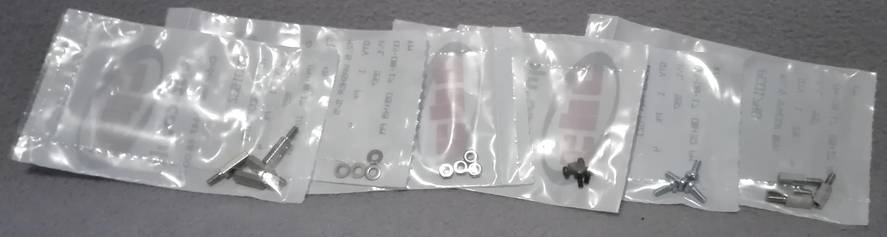
\includegraphics[width=0.9\linewidth]{photos/screws1.png}
    \caption*{Śrubki do zastosowań wewnątrz modelu}
\end{figure}
\begin{figure}[H]
    \centering
    \begin{subfigure}{0.32\textwidth}
        \centering
        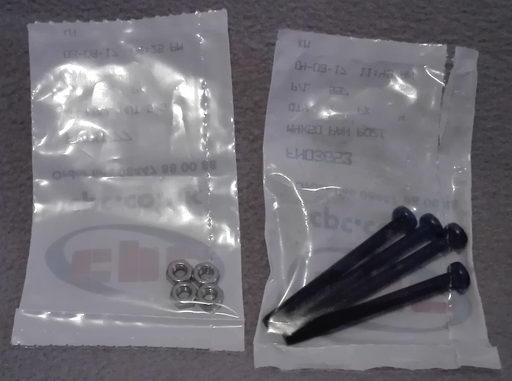
\includegraphics[width=0.9\linewidth]{photos/screws2.png}
        \caption*{Duże śrubki do spięcia modelu}
    \end{subfigure}
    \begin{subfigure}{0.32\textwidth}
        \centering
        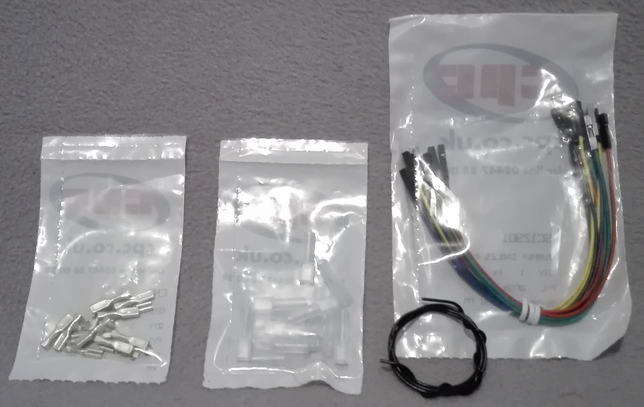
\includegraphics[width=0.9\linewidth]{photos/cables.png}
        \caption*{Zestaw kabelków, złącz i gumowych osłonek}
    \end{subfigure}
    \begin{subfigure}{0.32\textwidth}
        \centering
        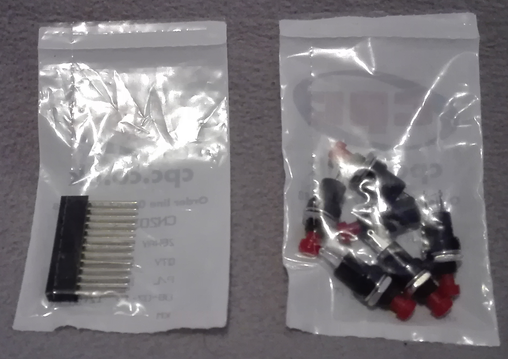
\includegraphics[width=0.9\linewidth]{photos/buttons.png}
        \caption*{Podwyższające złącze szpilkowe i przyciski}
    \end{subfigure}
\end{figure}

\section{Drukowanie}\label{sec:cover_printing}

Skorzystaliśmy z drukarki 3D znajdującej się w budynku Katedry Informatyki Akademii Górniczo
Hutniczej (KI AGH), by wydrukować elementy obudowy. Dostarczone w formacie stl schematy
przekonwertowaliśmy na format gcode rozumiany przez drukarkę.

\begin{figure}[H]
    \centering
    \begin{subfigure}{0.24\textwidth}
        \centering
        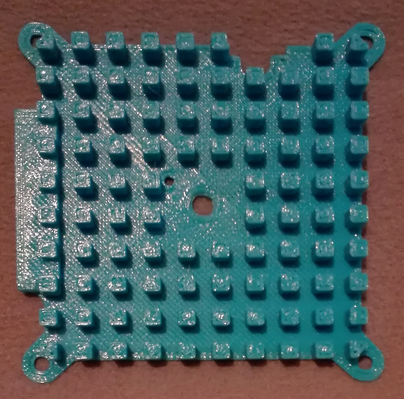
\includegraphics[width=0.9\linewidth]{photos/part1.png}
        \caption*{Radiator}
    \end{subfigure}
    \begin{subfigure}{0.24\textwidth}
        \centering
        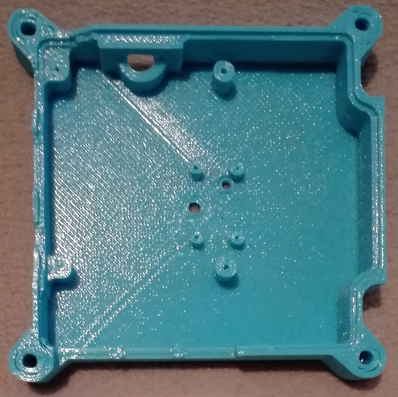
\includegraphics[width=0.9\linewidth]{photos/part2.png}
        \caption*{Podstawa}
    \end{subfigure}
    \begin{subfigure}{0.24\textwidth}
        \centering
        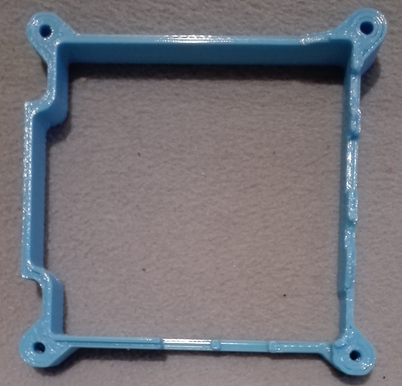
\includegraphics[width=0.9\linewidth]{photos/part3.png}
        \caption*{Środek}
    \end{subfigure}
    \begin{subfigure}{0.24\textwidth}
        \centering
        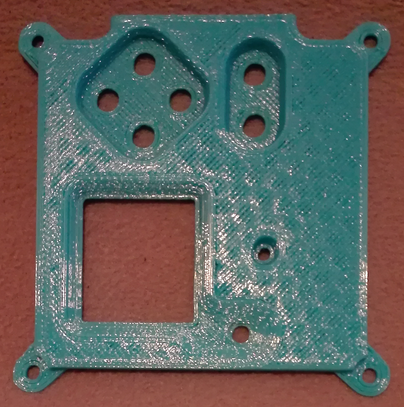
\includegraphics[width=0.9\linewidth]{photos/part4.png}
        \caption*{Panel główny}
    \end{subfigure}
\end{figure}

Każdy ze schematów dostarczony był w dwóch wersjach: normalnej i specjalnej na drukarki
gorszej jakości, które nierównomiernie ostygają. Asekuracyjnie wybraliśmy wersję drugą,
co okazało się błędem, ponieważ drukarka w budynku KI ostyga równomiernie i elementy
dodatkowe które miały w założeniu pomóc stygnąć, a później zostać oderwane, skleiły
się na stałe z modelem. Modelu tego ostatecznie nie wykorzystaliśmy przed błąd drukarki
który pojawił się pod koniec drukowania, a kolejne elementy drukowaliśmy już w wersji normalnej.

W trakcie drukowania natrafiliśmy na kilka problemów:
\begin{itemize}
    \item niezidentyfikowany błąd zatrzymał drukarkę w trakcie drukowania, a gorąca głowica
    stopiła jedną z nóżek drukowanego radiatora
    \item podczas drukowania ścianek bocznych ustawiliśmy zbyt małą prędkość drukowania,
    przez co ścianki drukowały się zbyt dokładnie i warstwy się nie połączyły, a ścianka
    rozwarstwiła
    \item uszkodzony fragment filamentu zaciął drukarkę, którą częściowo musieliśmy rozebrać,
    aby wyjąć uszkodzony fragment
\end{itemize}

W poradnikach drukowania znaleźliśmy informacje, że im mniejsza prędkość drukowania tym lepiej,
bo modele wychodzą dokładniejsze. Eksperymentalnie nauczyliśmy się, że dokładniejsze modele wcale
nie muszą być lepsze. Przez zbyt dokładne drukowanie ścianek zamiast jednej solidnej ścianki otrzymaliśmy
pięć pojedyńczych warstw zbudowanych jedna obok drugiej, które przez brak połączenia były bardzo kruche.

Mimo wszystkich przeciwności ostatecznie wydrukowaliśmy wszystkie elementy i zbudowaliśmy obudowę dla
mikrokomputera Raspberry.

\begin{figure}[H]
    \centering
    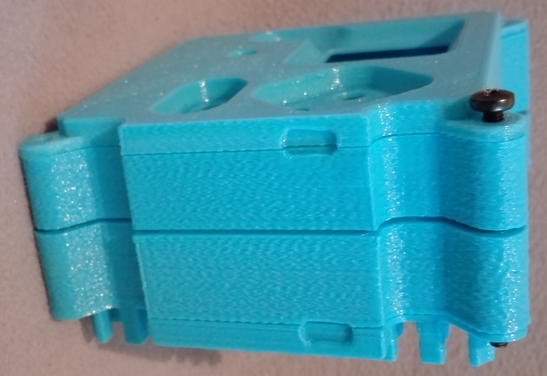
\includegraphics[width=0.6\linewidth]{photos/all.png}
\end{figure}
